\documentclass[a4paper,11pt,fleqn]{report}

\usepackage{acronym}
\usepackage{amsmath,amssymb,amsfonts}
\usepackage{booktabs}
\usepackage[dvipsnames]{xcolor}
\usepackage[margin=28mm]{geometry}
\usepackage{graphicx}
%	\graphicspath{
%		{.../Graphics/}
%	}
\graphicspath{{graphics/}}
\usepackage{hyperref}
	\hypersetup{
		colorlinks=true,
		linkcolor=blue,
		filecolor=blue,
		urlcolor=blue,
		citecolor=blue
	}
\usepackage[sort&compress]{natbib}
	\bibliographystyle{apalike}
%\usepackage[mark]{gitinfo2}
%\renewcommand{\gitMark}{Branch:\,\gitBranch\,@\,\gitAbbrevHash{}; Author:\,\gitAuthorName; Date:\,\gitAuthorIsoDate~\textbullet{}}
\usepackage{url}

\begin{document}
%===============================================================
% Frontmatter and title page to be added manually at the end
%===============================================================
\thispagestyle{empty}
\begin{center}
{\huge \textit{`e-casa'} - Eco-friendly Household Waste System\\Part II}
\vspace{20mm} \\
{\Large Group 6}
\vfill

A project report in partial fulfilment of the requirements for the subject\\
\vspace{10mm}
{\Large \textsc{Systems Engineering (BSS 410)}} \\
\vfill
%
in the \\
\vspace{20mm}
%
{\Large \textsc{Faculty of Engineering, Built Environment, and \\ 
Information Technology}}\\
%
\vspace{10mm}
{\Large\textsc{University of Pretoria}} \\
%
\vfill
%
\today
\end{center}

\textit{`e-casa'} - Eco-friendly Household Waste System
\pagenumbering{roman}

\chapter*{Executive Summary}
The aim of this project is to create a household waste management system of that will not only reduce the waste produced by a generic household but do so by increasing value to the user. The final deliverable for this project will be a report that details the needs analysis, conceptual design, feasibility and risk assessment of the designed system. The coneptual design will be done with the use of \textit{Core 9} to capture all identified needs accurately and produce system design documentation.

\tableofcontents
\listoffigures\addcontentsline{toc}{chapter}{List of Figures}
\listoftables\addcontentsline{toc}{chapter}{List of Tables}

\chapter*{Acronyms}
\addcontentsline{toc}{chapter}{Acronyms}
\begin{acronym}[ABCDEF]
\acro{e-casa}{Eco-friendly Household Waste System}
\acro{FBD}{Functional Block Diagram}
\acro{SD}{System Dynamics}
\end{acronym}

\chapter{Introduction and Background}
\pagenumbering{arabic}
\setcounter{page}{1}
\acresetall

\section{Problem Background} \label{sec: Problem Background}
Households consume a variety of products and create different wastes. Products may take the form of food items, municipal water, electricity and other consumables which are either used up or discarded after use. Products discarded after use, such as excess food, food and beverage packaging and water exit the household as forms of waste.  Food clippings from preparing dinner or paper-based packaging is often discarded into dustbins alongside plastic and other waste types to be collected and transported to a dump site. Water used at bathroom sinks or showers is sent directly to the the municipal water system after use to be disposed of. Each type of waste generated by a typical residential household requires proceeding systems that will either store, repurpose or discard the waste.
  
Recent trends have made the consumer market ecologically aware of their own waste generation and many systems have been created to reduce the total waste output of a household. Such products include grey water systems, recycling bins and compost containers. There is a growing need for these means to be adpoted but presently no solution on the market that integrates all means into one comprehensive system for homeowners.
  
Because these systems operate independently, the outputs of one system are often not used as inputs to another. Integrating these systems to operate together could provide more value to the user and further reduce household waste. For example: using food clippings (to create a compost heap) and grey water to grow vegetables in one's garden instead of disposing food clippings in a general waste bin and discarding water to the municipal water system directly after its first use. This eliminates the need for compost to be purchased from a store and reduces water consumption.

\section{Project Objective} \label{sec: Project Objective}
The objective of this project is therefore to investigate the possibility of integrating these different systems as one. The intention is to determine whether the potential cost and resource use savings to be earned from such an integrated system outweigh the financial cost and initial inconvenience to install.

\chapter{Concept Development Stage}
\section{Needs Analysis Phase} \label{sec: Needs Analysis Phase}
\subsection{Operational Need Analysis} \label{Ssec: Operational Need}
\ac{e-casa} is a sustainable household waste management system intended to fulfuill the increasingly prevalent need for sustainable living. The need for individuals and households to consume and dispose of resources in a more sustainable manner is becoming ever more pertinent because of increasing strain on the world's most essential natural resources such as water and fossil fuels. The need is driven by the requirement for individuals (and society as a whole) to reduce their negative impact on the environment by re-use, recycling and minimising resource use as these natural resources become more scarce. Successfully meeting this need will not only improve living conditions for societies but importantly alleviate pressure on governments and municipalities who have to manage and distribute these water and electricity resources to the public.
Although regulation does not yet fully drive this need, government encourages and sometimes imposes restrictions to encourage responsible water and electricity use. This is important to develop a sustainable mindset and awareness of waste generation. Because regulation is still limited on the use of these resources, the onus lies with society and individuals who are aware of and want to mitigate their negative impact on the environment.

\ac{e-casa} is aimed at fulfilling the operational need of sustainable living for households by providing a system that makes it possible to manage and dispose of waste responsibly while simultaneously minimising water consumption. \ac{e-casa} is also expected to provide long-term financial benefits to the user in the form of reduced water consumption costs and grocery bills (with some homegrown foods). Furthermore, there is the expected intangible benefit of the system - knowing one's adverse impact on the environment is mitigated.

Due to a lack of solutions currently on the market, there is an opportunity to enter a gap in the market with \ac{e-casa}. However, this gap is anticipated to be small in size as this product will mainly be aimed at high income individuals aware of (and wanting to reduce) their impact on the environment. There is also an opportunity to market this system as a product to middle class individuals who have sufficient capital to purchase such a system now in order to reap the aforementioned financial savings down the line. However, this extension will likely only be possible if the initial cost of the system is not too high for these individuals and the financial savings are substantial enough to persuade this group.\\


\subsection{Operational Objectives}
The overarching objective that \ac{e-casa} is intended to fulfil is to provide sustainable household waste management. This objective is deconstructed into three primary objectives, namely: \textit{Provide Waste Sortation and Storage}, \textit{Reduce Water Consumption} and \textit{Provide long-term cost savings}. Figure~\ref{fig: ecasaOT} shows the operational objectives of the \ac{e-casa} system.\\

\begin{figure}[h!]
\begin{center}
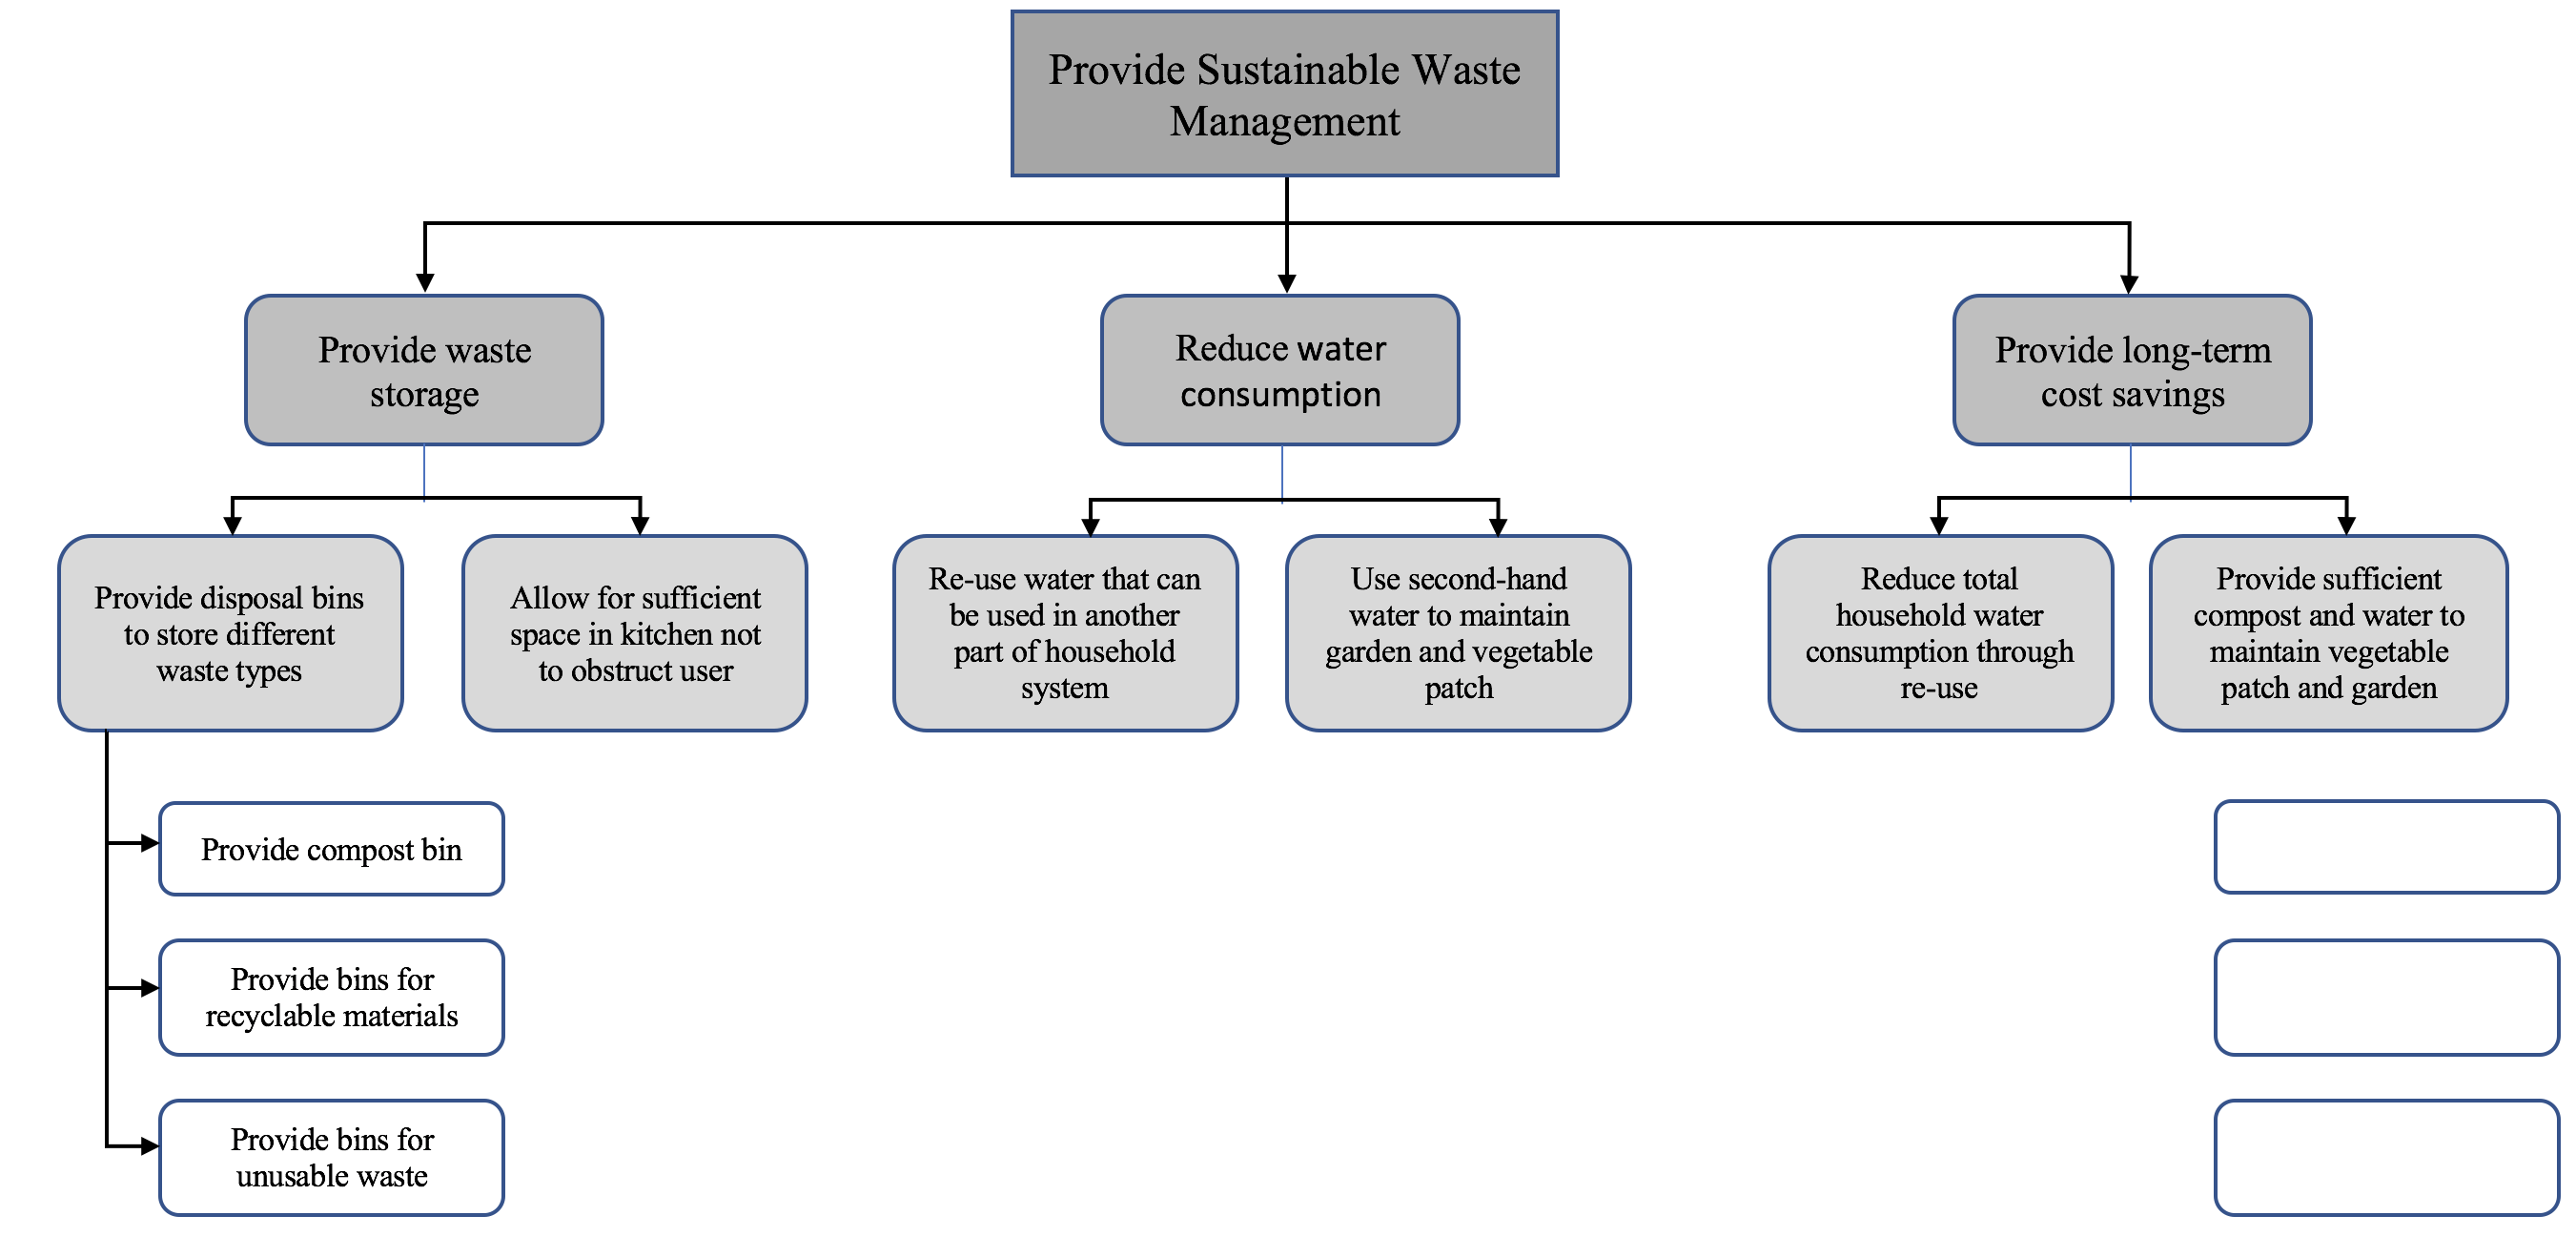
\includegraphics[scale = 0.55]{ecasa_OT.png}
\caption{e-casa Objective Tree Structure}
\label{fig: ecasaOT}
\end{center}
\end{figure}

\subsection{Functional Definition}
\ac{e-casa} needs to perform the following functions in order to achieve the objectives layed out in the objective tree:\\

\noindent\textbf{Provide Waste Sortation and Storage} - The system must provide the capability for waste to be sorted according to its composition: paper, plastic, glass, organic material and unusable waste. Organic material must be reatained to be used in a composter and recyclable waste stored temporarily in its respective category for it to be later removed from the household system and passed on to the local municipality waste collection service.\\

\noindent\textbf{Reduce Water Consumption} - To achieve this objective a grey water system will need to perform the functions of receiving used water, processing this water (to be re-used again), storing the water until it is demanded at an outlet and directing the water from storage to the necessary outlet when it is demanded.\\

\noindent\textbf{Provide Long-term Cost Savings} - The use of a grey water system alone will provide long-term cost savings by means of reduced water consumption. Therefore if the objective of reduced water consumption is met with a grey water system that fulfills the necessary functionality, the household will demand less water from the municipality and cost savings will be realised immediately during system use. However, to provide long-term cost savings in other terms, \ac{e-casa} will need to effectively integrate grey water, composting and waste recycling to use each other's outputs as inputs and reduce the amount of external resources such as compost, vegetables and water to required to be used as inputs to the household system.

Effective utilisation (re-use) of water and organic waste will reduce the amount of water that needs to be purchased from the municipality, compost that needs to be purchased and eventually groceries that need to be bought. This functionality is essential to reduce the household's input costs and provide tangible finanacial value to the system user.

\subsection{Feasibility Definition}
At present there are household recycling bins available on the market that separate waste into the necessary categories. The technology is therefore currently available and feasible as a solution to the functions of waste sortation and storage. A recycling bin similar to that shown in Figure~\ref{fig: Household separation recycling bin} would likely be purchased and used in the \ac{e-casa} system.

\begin{figure}[h!]
\begin{center}
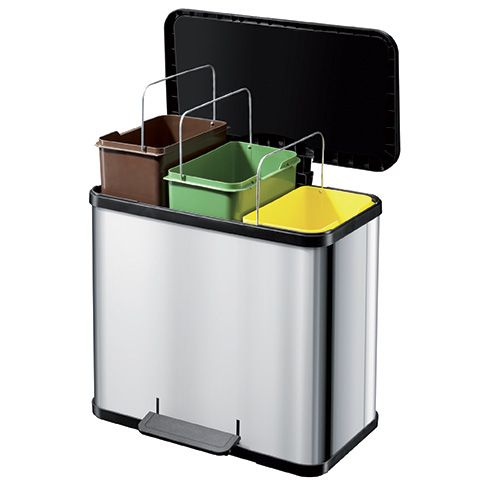
\includegraphics[scale = 0.34]{HouseholdRecyclingBin.jpg}
\caption{Household separation recycling bin, \citep{Rbins2018}}
\label{fig: Household separation recycling bin}
\end{center}
\end{figure}

There are also existing grey water systems available for purchase online or in-store. However, the setup of these systems and the size of its components usually vary case-to-case dependent on the appliances to be linked to the system, the size of the storage tank required by the household and the quality of the filtration component to be installed. Components of a grey water system can be easily purchased by any individual, but some degree of expertise and knowledge in the field is usually required to correctly size components, determine how they will function together and physically setup the system with the household's present water supply system. 

The design for \ac{e-casa}'s expected to be much like the one in Figure~\ref{fig: Grey water system} as it will be linked to the household's shower/bath, basins, washing machine, outdoor tap and toilet.
%
\begin{figure}[h!]
\begin{center}
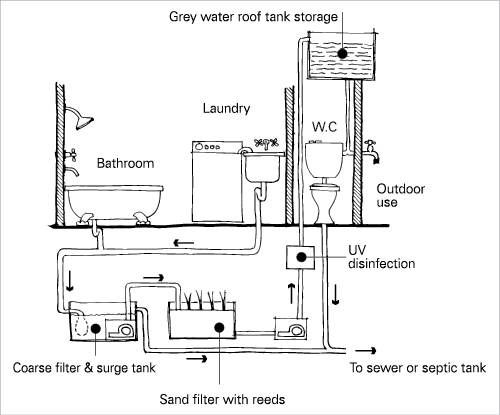
\includegraphics[scale = 1.2]{Household_Grey_Water.png}
\caption{Household grey water system, \citep{AuGov2013}}
\label{fig: Grey water system}
\end{center}
\end{figure}
%
A number of different household composters are available on the South African market. These composters are easily accessible and available online and in hardware stores. It is assumed for the time being that a 220 \textit{litre} composter (shown in Figure~\ref{fig: Outdoor Composter}) will be of sufficient size to store a household's organic and garden refuse waste.
%
\begin{figure}[h!]
\begin{center}
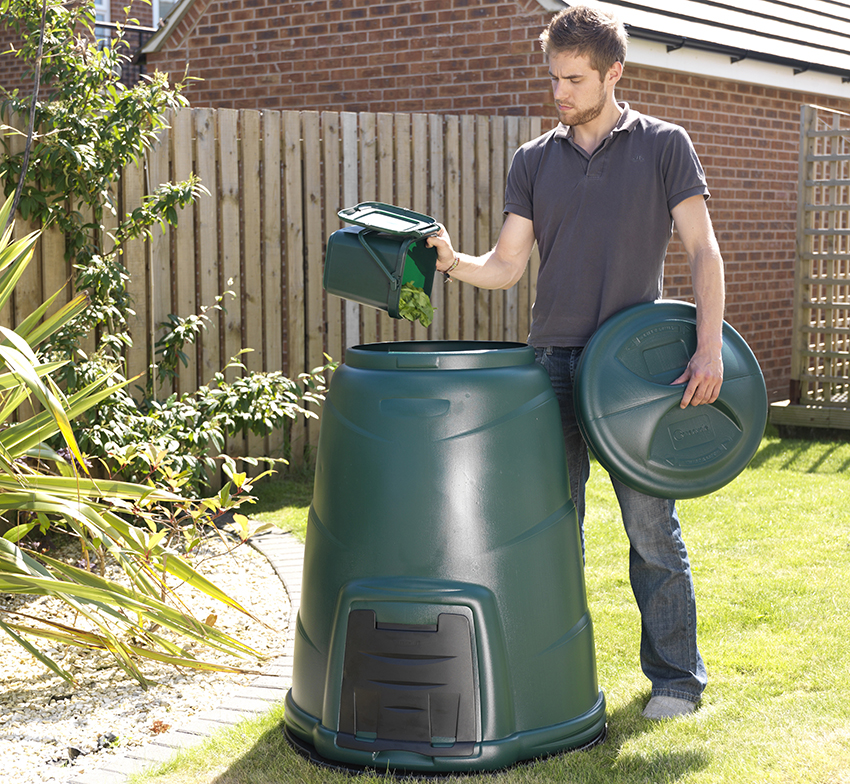
\includegraphics[scale = 1.1]{Outdoor_Composter.jpg}
\caption{Outdoor Residential Composter (220 \textit{litres}), \citep{FDB2018}}
\label{fig: Outdoor Composter}
\end{center}
\end{figure}

\subsection{Need Validation}
To ensure the proposed system can fufill the identified need, metrics have been developed that will be used to evaluate the performance of the system.
%
\begin{table}[h!]
\caption {System Performance Metrics} \label{tb: Performance_Metrics} 
\begin{center}
\begin{tabular}{p{5cm}|p{3cm}|p{8cm}}\toprule
	{\textbf{Metric Category}} & {\textbf{Unit Measure}} & {\textbf{Description}}\\ \midrule
    Water savings & \textit{litres} & The volume of water saved is calculated as the reduction in the volume of water that enters the household. This value is already measured by the household's municipality that bills them for water usage each month.\\
    \hline
    Organic waste reduction & \textit{kilogram} & The total mass of organic waste re-used by means of composting is the reduction in household waste output.\\
    \hline
    Disposable waste reduction & \textit{kilogram} & The total mass of plastic, paper and glass respectively represent disposal waste reduction. It is assumed firstly, that all disposable materials would not have been recycled before system implementation and secondly, that all disposable materials will ultimately be recycled by the municipality's garbage management system.\\
    \hline
    Household service cost saving & \textit{Rands} & The reduced water consumption of the household and the re-used organic waste helps to perform household activities that would otherwise require a homeowner to purchase more water, compost and vegetables. This includes the municipal water used in the household and compost for a vegetable garden. Household service cost saving is thus the total monetary savings obtained from reduced water use, self-composting and not having to purchase vegetables as frequently.\\
    \hline
    Payback Period & \textit{years} & The payback period is defined as the period of time it takes for the financial savings generated by the system, to equal the initial cost of purchasing and installing the \ac{e-casa} system. \\ \bottomrule
\end{tabular}
\end{center}
\end{table}
%
The five metrics in Table~\ref{tb: Performance_Metrics} are to be evaluated using different hypothetical scenarios. These scenarios reflect expected environmental conditions and consideration of the metrics in conjunction with these scenarios is used to determine the appropriateness of the system. The hypothetical scanarios are as follows:
%
\begin{description}
	\item[Municipal water restrictions] - If the local municipality decided to place water restrictions in the area of the household and the household's water use was currently above that threshold, the water savings metric would be used to determine whether the household could reduce their water consumption enough by installing the system to fall under the specified limit.
	\item[Equipment price rise] - If the price of grey water system equipment rises substantially due to unfavourable economic circumstances or exchange rate changes before the \ac{e-casa} system is installed, the payback period will significantly increase as more capital would have to be earned back in the form of savings which would take a longer period of time.
\end{description}

The metrics are shown to be helpful in assessing the performance of the system under the different external operating conditions (hypothetical scenarios given above). 
%As defined by the metrics, the system is believed to achieve the objectives laid out by the defined need. Thus the system is able to fufill the identified needs.

\section{Concept Exploration}
\subsection{Operational Requirements Analysis}
The three primary objectives of the system are to reduce water consumption, provide waste sortation and storage, and to provide long-term cost savings. The following operational requirements are specified according to these three objectives: \\

\textbf{Water Consumption}
\begin{itemize}
\item Reduce Water Consumption
\item Grey water collection
\item Grey water storage 
\item Greywater filtration 
\item Filtered greywater diversion 
\end{itemize}
\medskip
\textbf{Provide Waste Sortation and Storage}
\begin{itemize}
\item Waste storage by type 
\item Visual compartment distinction 
\item Safe and odourless waste containment 
\item Specialised organic waste storage 
\item Compost to veggetable patch distribution 
\end{itemize}
\medskip
\textbf{Provide Long-term Cost Savings}
\begin{itemize}
\item Water volume usage reduction
\item Garden maintenance cost reduction 
\item Self-grown vegetables from garden
\end{itemize}

\subsection{Performance Requirements Formulation}
Subsystem functions are defined and allocated from the operational requirements discussed above and can be found in the following \ac{FBD}s:\\ 
%
\begin{figure}[h!]
\begin{center}
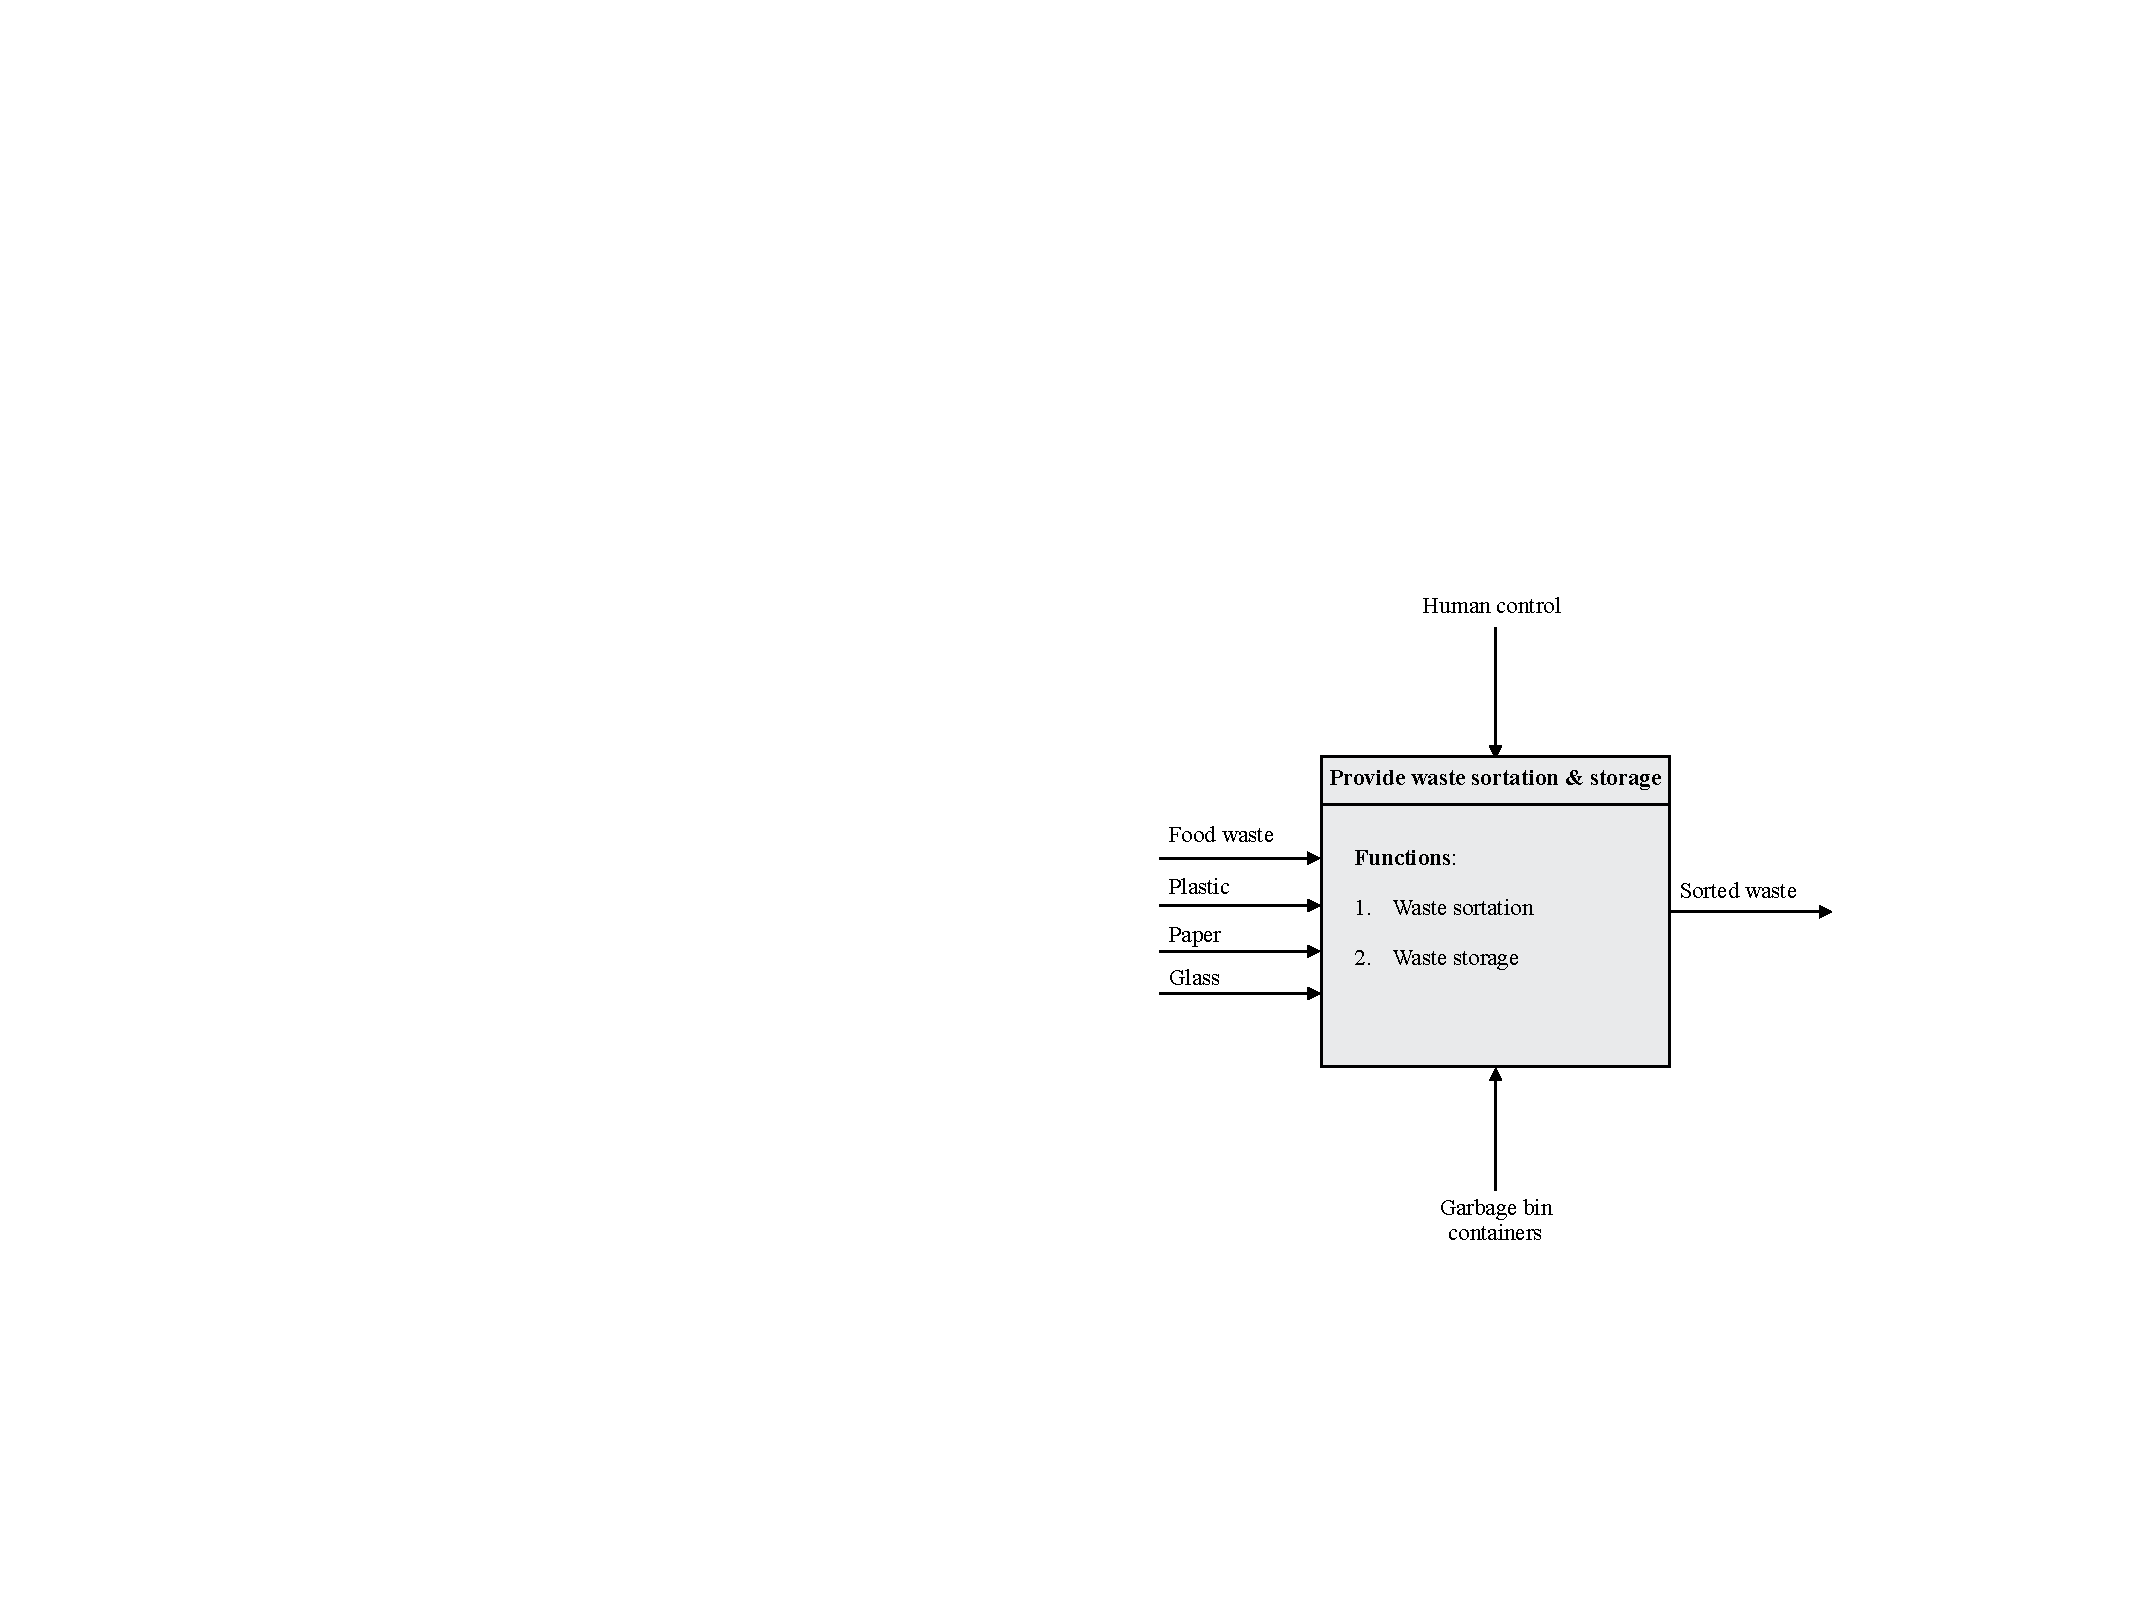
\includegraphics[scale = 0.4]{Function1.pdf}
\caption{Function 1: Provide waste sortation and storage}
\label{fig: Function1}
\end{center}
\end{figure}
%
\begin{figure}[h!]
\begin{center}
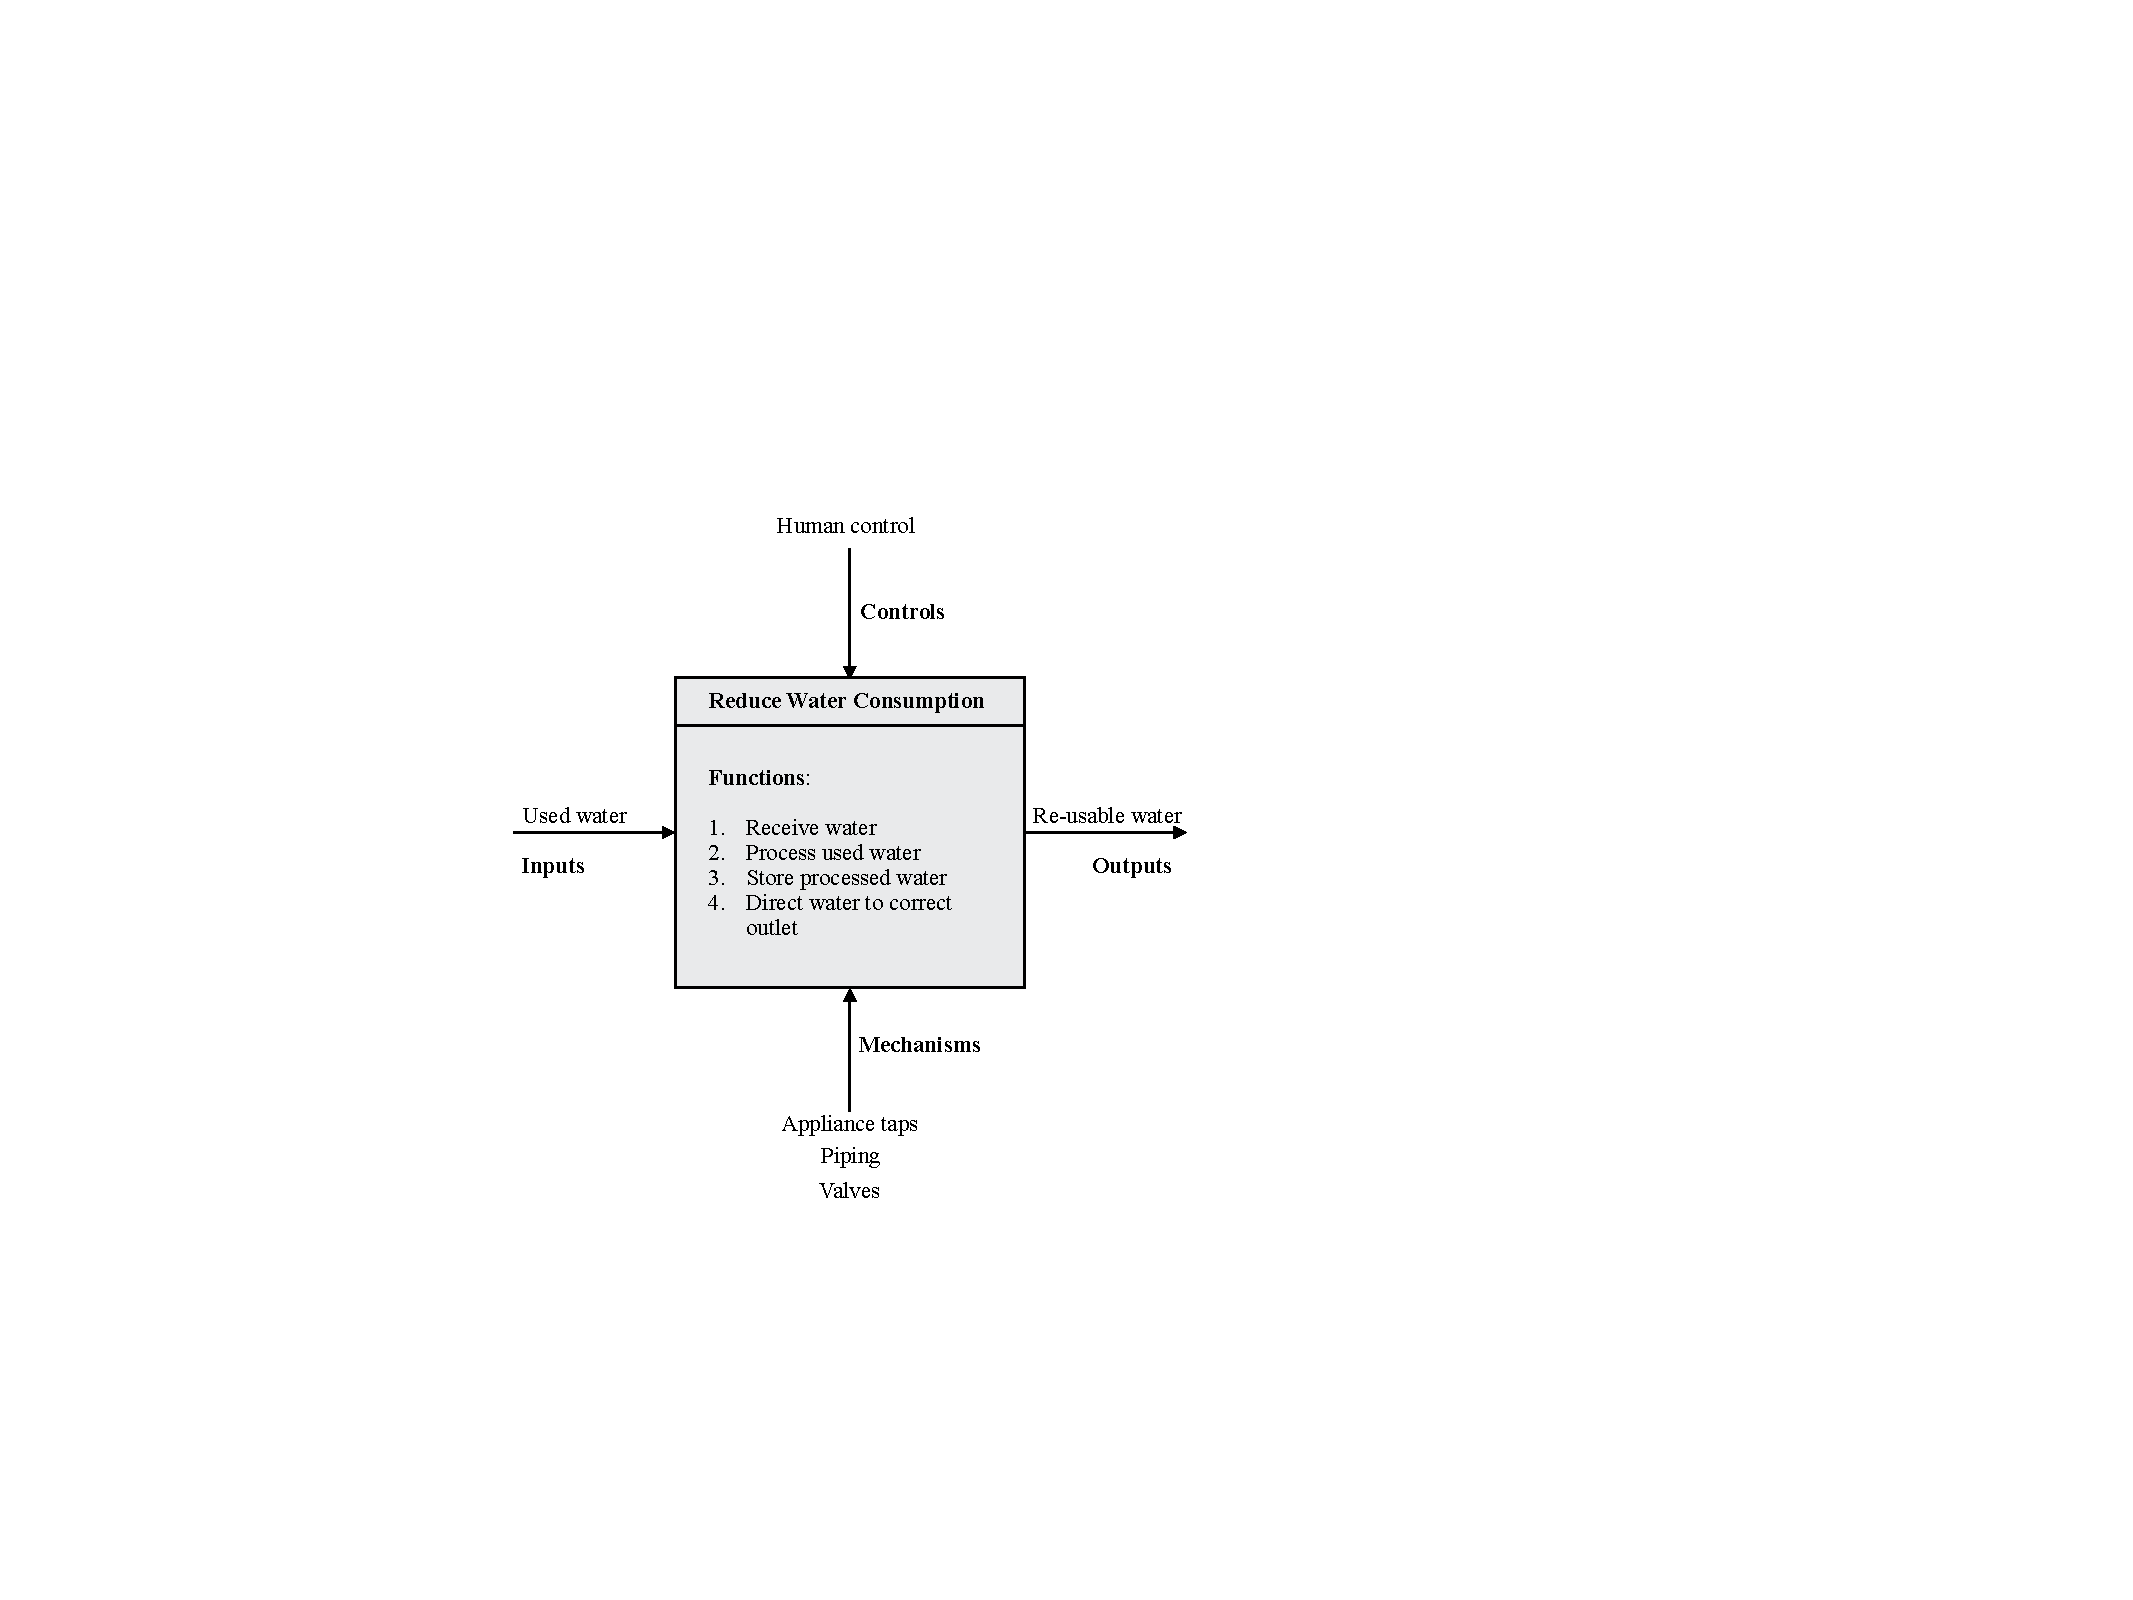
\includegraphics[scale = 0.8]{Function2.pdf}
\caption{Function 2: Reduce water consumption}
\label{fig: Function2}
\end{center}
\end{figure}
%
\begin{figure}[h!]
\begin{center}
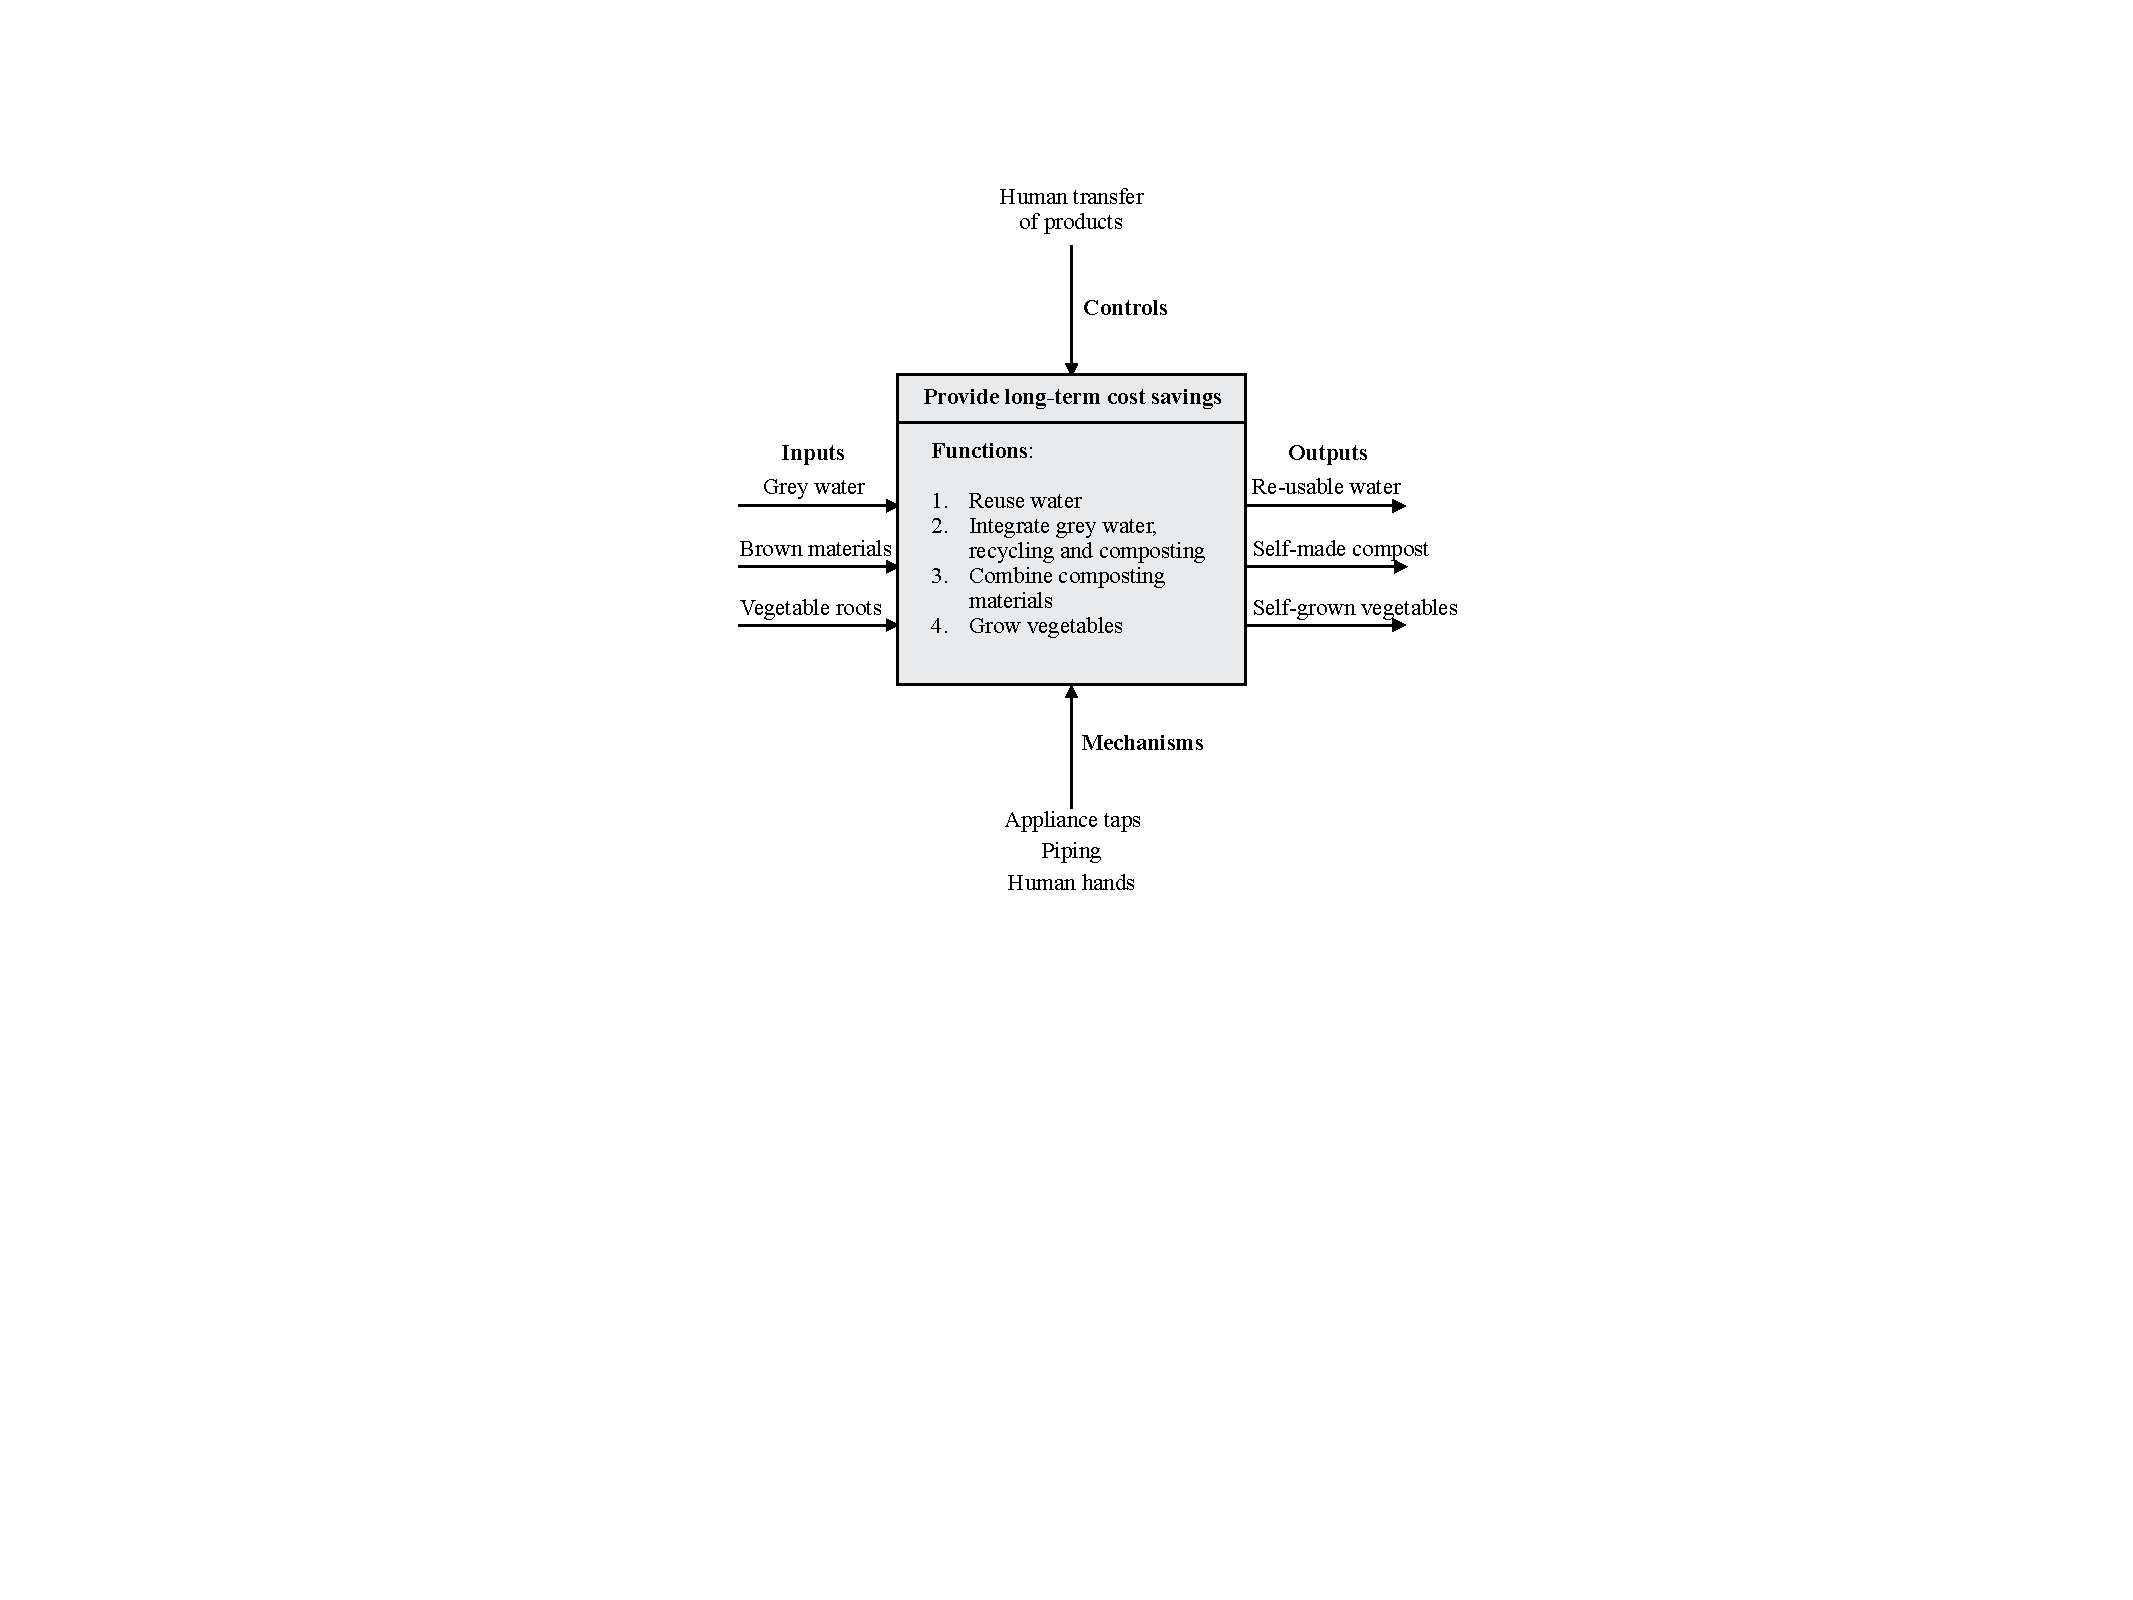
\includegraphics[scale = 0.8]{Function3.pdf}
\caption{Function 3: Provide long-term cost savings function}
\label{fig: Function3}
\end{center}
\end{figure}

\subsection{Implementation of Concept Exploration}
Multiple alternatives for each of the function tasks given in \ac{FBD}s are explored in Table~\ref{tb: FunctionalTasks}.
%
\begin{table}[h!]
\caption {System Alternatives for Functional Tasks} \label{tb: FunctionalTasks} 
\begin{center}
\begin{tabular}{p{3.5cm}|p{6cm}|p{6cm}}\toprule
	{\textbf{Functional Task}} & {\textbf{Alternative 1}} & {\textbf{Alternative 2}}\\ \midrule
    Waste sortation and storage & One garbage bin with multiple compartments & Multiple garbage bins each with a single compartment\\
    \hline
    Receive water & Four separate pipes from (bath, shower, basin and washing machine) that connect to the central grey water storage tank & One pipe that merges bathroom appliance outputs and one for the kitchen. These two pipes will feed water to the central grey water tank\\
    \hline
    Process used water & Filter grey water to be sent back to the washing machine for re-use and to the garden (for composting and plant watering) and toilet cistern (for flushing) & Do not purchase a filter and only use grey water in the garden and to flush the toilet cistern\\
    \hline
    Store processed water & Large central tank to store all water received until it is needed again by the washing machine, toilet cistern or in the garden & Smaller central tank to store used water only for use in the garden\\
    \hline
    Direct water & Five-way water valve to direct grey water back to the washing machine, to an outside water tap (to be used in a compost container), to the garden's sprinkler system (to water the vegetable patch) and to the toilet cistern & Three-way valve to direct grey water back to outside water tap to be used in a compost heap and to the garden's sprinkler system to water the vegetable patch\\
    \hline
    Re-use water & Grey water system makes water available for re-use at necessary outlet points when human user demands it at a tap & Grey water system makes water available for re-use at necessary outlet points in the required quantities (specifically at the garden's sprinkler system to eliminate the need for the user to retrieve the water and use it themselves)\\
    \hline
    Integrate water, recycling and composting & N/A - Alternatives explored by other system functions & N/A - Alternatives explored by other system functions\\
    \hline
     Combine composting materials & Purchase a residential size compost container that the necessary materials are combined in to produce compost & Create a large compost heap in the household's garden to store and mix compost materials. Construct a structure to shelter this compost and fix it in place\\
    \hline
     Grow vegetables & User must collect water from the outside garden tap in the necessary quantity and use it to water the vegetable patch. Compost collected and filled in the vegetable patch manually by human user & Connect grey water storage tank directly to garden sprinkler system to be activated by the human user at the flick of the sprinkler switch. Compost collected and filled in the vegetable patch manually by human user\\
    \hline
    \bottomrule
\end{tabular}
\end{center}
\end{table}
%
	
\subsection{Performance Requirements Validation}

\section{Concept Definition}
\subsection{Performance Requirement Analysis}
\textbf{System performance requirements refinement} - The system performance requirements do not consider the impact the size of the household may have on them and are these performance requirements are rather set using data for an “average” household in South Africa. The size of the household will affect the size of the required system, the cost of such a system and therefore the system’s ability to be financially feasible. The waste producing capacity of a smaller household is a constraining requirement as smaller households will produce less waste and it will take longer to realise the cost savings of a larger system (possibly more than 2 years). However, smaller households will require smaller system components and therefore a lower initial system cost than a larger system. Additional constraint requirements are also to be included that specify the minimum household size for the system to be feasible.

To ensure the long-term operation of the system, each subsystem must be made easy for the system user him/herself or cheap labour to maintain. Standardised components are therefore preferred for the greywater system as well as the physical waste system. \\

\noindent\textbf{Updated performance requirements} -
The following performance requirements were included in the specification after reviewing the initial performance requirements.\\

\begin{table}[h!]
\caption {System Performance Requirements} \label{tb: Functional_SS_elements} 
\begin{center}
\begin{tabular}{p{3cm}|p{6cm}|p{5.5cm}}\toprule
	{\textbf{Output}} & {\textbf{Performance Description}} & {\textbf{Specification}}\\ \midrule
    \hline
   Waste sortation and storage & Capacity to handle household's disposable waste for week before recycling bin containers need to be emptied  & 2.1 kg paper, 3 kg plastic, 1.8 kg glass, \citep{Sithole2014}\\
        \hline
    Re-usable water & System must be able to be able to supply a certain (\%) of household appliance water demands with grey water & ?\\
        \hline
    ... & ... & ...\\
        \hline
    ... & ... & ...\\
        \hline
    ... & ... & ...\\
        \hline
    ... & ... & ...\\

    \bottomrule
\end{tabular}
\end{center}
\end{table}

\noindent\textbf{Relating analysed specifications to operational needs}\\

\noindent\textbf{Reduce water consumption}
\begin{enumerate}
\item To reduce the amount of water consumed by the household, water from the bath, shower, basin and washing machine will be re-used. The water is diverted to toilet cisterns and into the veggie patch or garden. The specification for this function is that the households total water consumption will reduce by at least 147 l per day (33\%) (this is all water used by the showers, baths and washing machine then re-used for garden or toilet flushing purposes). The grey water system can divert a sufficient volume of water back into the house for consumption or this water can be stored for later use. The net effect is that less water is purchased from the municipality and the household consumption decreases thus satisfying the requirement.
\end{enumerate}

\noindent\textbf{Reduce the amount of physical waste sent to landfills}
\begin{enumerate}
\item Disposable waste refers to the mass of plastic, paper and glass generated by the household, received by the municipality and sent to landfills.The system should reduce this value by at least 1.44 kg per household per week (90\%). To achieve this, e-casa either uses the physical waste or sorts it for a third party, excluding the municipality, to process. 
\item Organic waste is composted within the e-casa system and re-used in the vegetable patch, replacing the need for fertilisers to be purchased. The system aims to reduce the amount of organic waste sent to landfills by at least 3 kg per household per week (90\%)Recyclable waste, such as paper or glass, is stored separately from hazardous and plastic material. In both instances, the mass of physical waste being transferred to the municipality is lowered reducing the production of physical waste.
\end{enumerate}

\noindent\textbf{Provide sustainable waste management system}
\begin{enumerate}
\item Reducing the amount of water consumed by a household directly reduces running costs, and any reduction in water consumption will therefore realise a cost saving for the system user. The estimated cost saving per year was calculated as 147 l/day. With a rate of R18.97 per kl this translates to a savings of R1018 per year.
\item The reduction in costs generated by the composting subsystem will only be realised once the composting process is complete, this is expected to take a minimum of 3 months. If this compost replaces store bought compost a savings of R1 per litre can be realised. Using 3 kg of organic waste per week a total savings of R195 can be realised per year. The self-produced compost can then be used to grow vegetables, causing further estimated savings of R456 per year to be realised in the form of reduced grocery costs for the household, given a 2 square meter garden and a benchmark cost for vegetables.
\item The specification for the payback period metric is 7 years, meaning cost savings generated by the system must pay back the initial cost of the system within a  7 year period.
\item Reducing the water consumption and physical waste generation (through recycling and re-use) lessens the the negative impact on the environment. A specification of 30\% reduction in total waste output for a household within a year period will significantly reduce the waste accumulated in local landfills, thus reducing the impact on the environment.
\end{enumerate}

\subsection{Functional Analysis and Formulation} 
Each subsystem is summarised along with its class of function, element function and the physical elements required to perform the function in Table~\ref{tb: Functional_SS_elements}.\\

\begin{table}[h!]
\caption {Functional subsystem elements} \label{tb: Functional_SS_elements} 
\begin{center}
\begin{tabular}{p{3.5cm}|p{3cm}|p{3cm}|p{4cm}}\toprule
	{\textbf{Subsystem}} & {\textbf{Class function}} & {\textbf{Element Function}} & {\textbf{Physical Elements}}\\ \midrule
    Grey water & Material & Process used water & Piping, water storage tanks, valves, pump\\
    \hline
    Waste sortation and storage & Material & Sort waste, store waste & Separate bins, bags, garbage bin housing\\
    \hline
        Compost & Material & Generate compost & Storage container\\
    \bottomrule
\end{tabular}
\end{center}
\end{table}

\textbf{System walkthrough}: The following process details how the system will function in practice:\\

Water is used from the municipal source via taps, showers, baths, wash basins and washing machines. This water is diverted into storage tank. The remaining water used in toilets etc is sent into the sewage line. Water in the grey water storage tank is diverted into two paths. The first path filters and sterilizes the water for re-use in the washing machine. The second sends the remaining grey water into the either the toilet cistern or the garden.
Water diverted into the garden automatically irrigates the vegetable patch and garden. Physical waste produced by the house is sorted into useable and unusable waste. Usable waste is further divided into organic and inorganic waste. Organic waste
Garden refuse, and organic waste produced from the kitchen is transported to the composting system.
The organic waste is broken down into compost and used in the garden or in the vegetable patch.
The greywater from the greywater system is used to irrigate the veggie patch. Garden refuse is generated during this processes and is used as input into the composting system. Inorganic waste such as glass, plastic and paper enters the recycling system and is stored into demarcated bins. Once the bins reach full capacity, they are sent for recycling. Unusable waste
Hazardous material and non-recyclable material is disposed of in a traditional bin. The municipality receives the contents of the bin for further processing at a landfill.

\subsection{Concept Selection}
The alternatives given for the functions in Table~\ref{tb: FunctionalTasks} were assessed according to financial feasibility, convenience and ease of implementation. One alternative was selected for each function (Table~\ref{tb: chosen_Alts}) with the explanation for choice in each alternative given below:\\

\begin{table}[h!]
\caption {Functions and their selected alternatives} \label{tb: chosen_Alts} 
\begin{center}
\begin{tabular}{p{3.5cm}|p{9cm}}\toprule
	{\textbf{Function/Task}} & {\textbf{Selected Alternative}\\ \midrule
    Waste sortation and storage & One garbage bin with multiple compartments \\
     \hline
     Receive water & Four separate pipes from (bath, shower, basin and washing machine) that connect to the central grey water storage tank\\
    \hline
    Process used water & Filter grey water to be sent back to the washing machine for re-use and to the garden (for composting and plant watering) and toilet cistern (for flushing)\\
    \hline
    Store processed water & Large central tank to store all water received until it is needed again by the washing machine, toilet cistern or in the garden\\
    \hline
    Direct water & Five-way water valve to direct grey water back to the washing machine, to an outside water tap (to be used in a compost container), to the garden's sprinkler system (to water the vegetable patch) and to the toilet cistern\\
    \hline
    Re-use water & Grey water system makes water available for re-use at necessary outlet points when human user demands it at a tap\\
    \hline
    Integrate water, recycling and composting & N/A - Alternatives explored by other system functions\\
    \hline
     Combine composting materials & Purchase a residential size compost container that the necessary materials are combined in to produce compost\\
    \hline
Grow vegetables & Connect grey water storage tank directly to garden sprinkler system to be activated by the human user at the flick of the sprinkler switch. Compost collected and filled in the vegetable patch manually by human user\\
    \hline
    \bottomrule
\end{tabular}
\end{center}
\end{table}
%

\textbf{Recycling and waste disposal tasks}\\
For waste sortation, alternative one will be selected in order to save space and keep the garbage bin as small as possible to fit into the household's kitchen.\\

\textbf{Grey water tasks}\\
To receive water, the alternative with the least invasive way of changing the household's current piping system will be selected (which is anticipated to be ?). With regards to the processing of used water, alternative two will be selected. This is because the filter is a significant expense and will require frequent maintenance. The significant expense and inconvenience of alternative one is anticipated to outweigh its financial benefit as this would only save water being demanded by the household's washing machine.

Alternative two for used water storage goes hand-in-hand with alternative two for water processing. Because a filter will not be purchased for the grey water system, a smaller central tank will be used to temporarily store used water until it is demanded for vegetable garden and composting activities. Alternative one is chosen for the re-use water function. Water will be made available for re-use by the grey water system that will make it available at the outside garden tap and sprinkler system for the user. It is then up to the user to use (re-use) this water as best possible.

Alternative two would provide more value to the system user but would require substantial, research, financial investment and testing to develop and automated system that caters specifically to the household's unique needs. For the direct water function, alternative two will be selected as only a two-way valve will be needed if water is not to be re-directed from the storage tank to the washing machine for use.\\

\textbf{Financial savings related tasks}\\
The function of integrating water, composting and recycling will be performed both by hardware and the human user. Hardware (piping) will be used to connect the grey water subsystem directly to the outside sprinkler system surrounding the vegetable patch and to an outside tap for garden water usage. Grey water directed to the outside tap will need to be collected in the necessary quantity by the human user and input into the compost container. The human user will also be required to create the link between the recycling system and the compost system by means of physically transporting paper waste, garden refuse and food clippings to the compost container. There is no alternative for this option because alternatives for integrating these subsystems in different ways are explored through the other function tasks.

Alternative one will be selected to combine composting materials. Although a large garden compost heap may produce more compost than a smaller compost container, the smaller residential compost container is more convenient for the human user. To maintain a large compost heap in the garden (alternative two) is not practical for all households due to: space restrictions, the need for a structure to protect the compost from weather conditions that will change the balance of water in the heap and the cost of such a structure. The function of combining the composting materials will be performed by the human user who will place the required amounts of dry materials, food waste, paper and brown materials into the residential size compost container.

The task of growing vegetables will need to be performed by the human user. However, fulfilling this function will be made easier for the human user by selecting alternative two that will connect the household's water sprinkler system directly to the grey water storage tank. This way the user will just have to flick a switch to turn on the sprinklers and water the vegetable garden instead of manually collecting water from a tap and watering the growing vegetables. Although alternative two is expected to be more expensive because of the hardware required, it is expected to add a significant benefit to the system user in the form of convenience. The compost to grow vegetables will have to be collected out of the bottom of the compost container by the human user and placed into the vegetable patch. This is because there is not yet a way to automate this process feasibly on such a small scale.

The system as whole must be as cost effective as possible. However, quality should not be sacrificed for unreliable components. The grey water system components will be selected with the intention of a minimum 50 year project life for each, as per industry piping standards. \citep{Fischer2012}. This is important to ensure the system does not require large-scale repairs over the life of the project, only routine maintenance and reparis. The labour and expertise required to make system repairs for the installed grey water system are expected to be costly and should be avoided.

The selected alternative for each function will be chosen to form the final system.

\subsection{Concept Validation}
The system concept is validated by the following list of requirements:\\

\noindent\textbf{Physical waste management}
\begin{itemize}
\item Be sanitary
\item Not be odorous
\item Be as aesthetically pleasing as possible
\item Be small enough to fit in a kitchen
\item Be big enough to store one week's worth of recyclables
\item Be simply to use
\item Be child and pet safe
\end{itemize}

\noindent\textbf{Grey water management}
\begin{itemize}
\item Require minimal setup
\item Integrate with current infrastructure
\item Use standard piping for ease of maintenance and repair
\end{itemize}\\

\noindent\textbf{Composting and vegetable garden}
\begin{itemize}
\item Be self sustaining/ require minimal attention
\item Be able to produce own vegetables
\item Be aesthetically pleasing in the garden as possible
\item Be small enough to fit into an average size garden
\item Vegetable patch big enough to consume the compost produced
\end{itemize}\\

\noindent\textbf{Financial saving aspects }
\begin{itemize}
\item Be able to achieve payback period of 7 years
\end{itemize}\\

\chapter{Engineering Development Phase}
The system's functional specifications are translated into three subsystem functional requirements:\\

\textbf{Grey Water subsystem} - This system interfaces with the household's municipal water supply which is its primary input. It is also connected to multiple household components, namely: the washing machine, bath/shower, toilet cistern and garden. This subsystem has three functional capabilities. The first being to store grey water in a central tank to be recycled (re-used) in the system, secondly to sort re-usable water from unusable waste water and finally to transfer both the re-usable and unusable water in the subsystem to the appropriate destination (component). This subsystem also feeds grey water to the next subsystem (compost).\\

\textbf{Compost subsystem} -  The compost subsystem interfaces with the household's garden and organic material stockpile components. It uses organic materials from the material stockpile to provide compost to the garden component. It's primary capabilities are to store organic materials and provide some form of visual management for the user to know when there is sufficient compost for the storage container to be emptied. This subsystem is connected to the grey-water subsystem which provides grey water as an input as well as to the Recycling and waste disposal subsystem which provides paper and other organic waste to the compost system.\\

\textbf{Recycling and waste disposal subsystem} - This subsystem interfaces with the household's kitchen as a component in order to receive all household waste as an input. It also intrefaces with the municipal recycling system at the point where waste is placed on the sidewalk for collection by the municipality's waste collection service. Its primary capability is to sort household waste into the relevant categories for re-use or disposal. Paper recyclables and organic waste collected by this subsystem are output to be used in the compost subsystem while other recyclables and non-recylable waste is disposed of to the municipal recycling system.
%
\begin{figure}[h!]
\begin{center}
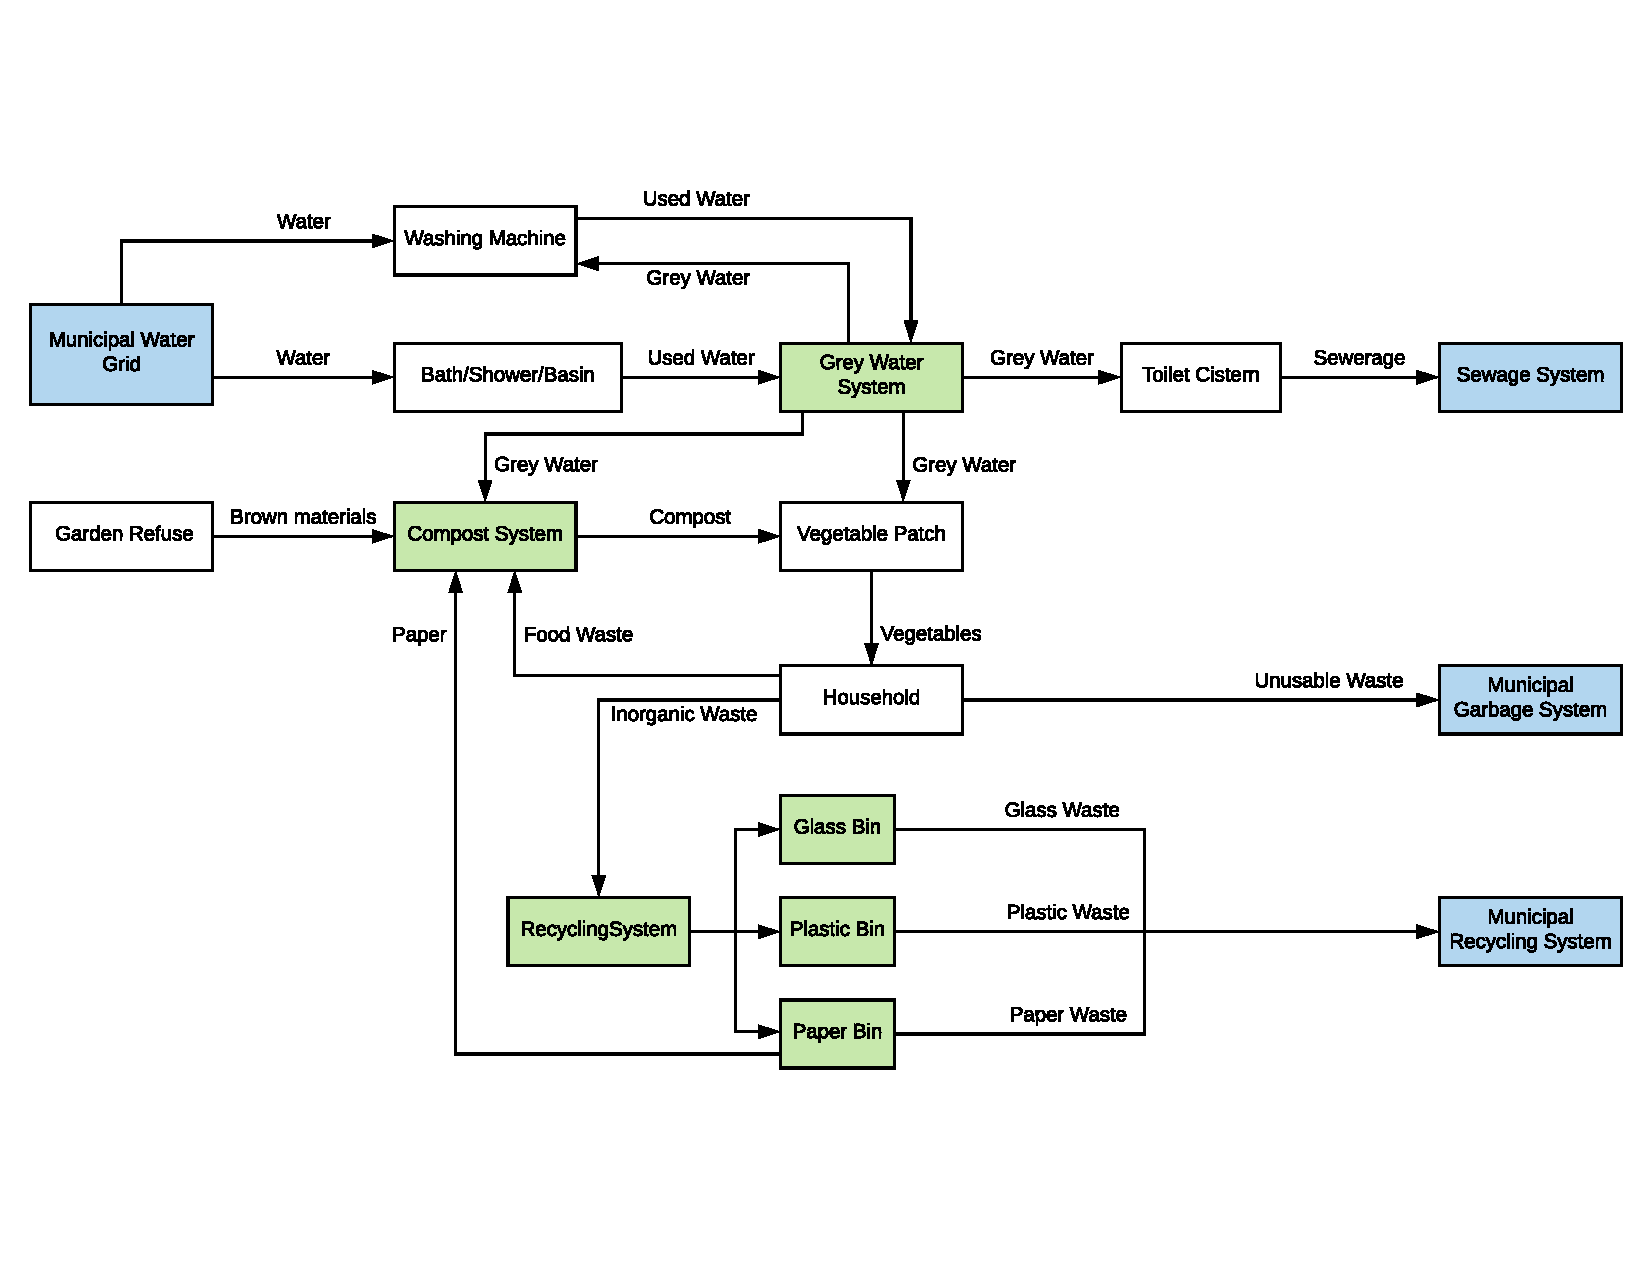
\includegraphics[scale = 0.55]{System_Diagram.pdf}
\caption{System Diagram}
\label{fig: systemDiagram}
\end{center}
\end{figure}
%
\section{Advanced Development Phase}
The components for the three aforementioned subsystems of \ac{e-casa} have already been designed and can be purchased from the market. The components will therefore not be evaluated individually but \ac{e-casa} is unique in that it is the first system of this kind that integrates these different components .
For this reason, the advanced development phase for the selected concept will be conducted to identify possible implementation risks of using these components together as one system.

\subsection{Prototype Development}
%
\begin{table}[h!]
\caption {Selected alternatives and their associated risks} \label{tb: Functional_SS_elements} 
\begin{center}
\begin{tabular}{p{7cm}|p{7cm}}\toprule
	{\textbf{Selected Alternative}} & {\textbf{Associated Risk}\\ \midrule
    \hline
    Single bin with multiple compartments & If a compartment or one part of the bin breaks, the entire bin needs to be replaced as individual parts are not sold separately.\\
        \hline
    Four separate pipes into the greywater system  & Installation may become complicated and thus more costly since more materials may be required.\\
        \hline
    Filter used water & Including a filter will increase the electricity usage and the cost of the overall system. Cleaning the filter may be an inconvenience to the user. If the filter pump breaks it may be costly to replace. \\
        \hline
   Large central greywater tank & The cost of the tank increases with larger size. If the water is treated incorrectly the effects will be experienced broadly by the household. \\
        \hline
    Five way water valve & If the valve gets blocked or breaks, all aspects linked to the system will be adversely affected. More connections means more widespread effect on the household.\\
        \hline
    Greywater available on demand from a tap & If all the greywater has been used on other areas of the household, the tap may run dry. Water that could otherwise be used for cooking and drinking will be used to water the garden. Manually transferring water may be an inconvenience for the user\\
        \hline
    Residential sized compost container & The above ground container can be knocked over by pets and wild animals.\\
        \hline
    Greywater system connected directly to sprinkler system & Additional parts will be needed to connect switches and electronic pumps. A malfunction in the sprinkler system could result in the garden not receiving water or excessive water usage. \\
    \bottomrule
\end{tabular}
\end{center}
\end{table}
%

\subsection{Development Testing}
Associated risks for each of the functions of the system are identified and appropriate mitigation plans suggested in Table~\ref{tb: Functional_risk_mitigation}.
%
\begin{table}[h!]
\caption {Associated risks and applicable risk mitigation plans} \label{tb: Functional_risk_mitigation} 
\begin{center}
\begin{tabular}{p{3cm}|p{5.5cm}|p{5.5cm}}\toprule
	{\textbf{Function} & \textbf{Associated Risk}} & {\textbf{Risk Mitigation}\\ \midrule
    \hline
    Waste sortation and storage & User places disposable waste into incorrect category (i.e. plastic into paper or paper into glass) & Use visual management signals or colours to mark garbage bin compartments clearly\\
      \hline
    Waste sortation and storage & If a compartment or one part of the bin breaks, the entire bin needs to be replaced as individual parts are not sold separately & Negotiate an agreement with the suppliers for cheaper prices or to order individual parts when required\\
     \hline
     Receive Water & Installation may become complicated and thus more costly since more materials may be required & The pipe layout should be standardised and the total volume of materials needed should be reduced through appropriate planning procedures\\
    \hline
Process Used Water & Including a filter will increase the electricity usage and the cost of the overall system. Cleaning the filter may be an inconvenience to the user. If the filter pump breaks it may be costly to replace & Ensuring that the filter is placed in an accessible location will allow maintenance to be carried out as conveniently as possible\\
    \hline
Store Processed Water & The cost of the tank increases with larger size. If the water is treated incorrectly the effects will be experienced broadly by the household & Ensuring that the tank is robust so that is does not break easily and making access to the tank easy can allow the water to be treated consistently well. Making the tank removable could allow it to be better cleaned and disinfected if necessary\\
    \hline
Direct Water & If the valve gets blocked or breaks, all aspects linked to the system will be adversely affected. More connections means more widespread effect on the household & A back up five-way valve could be included to take over if the original valve fails. Adding a tap before the valve can allow the water to be shut off so that the failed five way valve can be easily replaced\\
    \hline
Reuse Water & If all the greywater has been used on other areas of the household, the tap may run dry. Water that could otherwise be used for cooking and drinking will be used to water the garden. Manually transferring water may be an inconvenience for the user & A backup pipe can be linked from the municipal water system to the greywater system to become active when the tank is empty\\
    \hline
Combine Composting Materials & The above ground container can be knocked over by pets and wild animals & 
The above ground container can be knocked over by pets and wild animals. The container can be semi buried or strapped down to maintain stability. The container has a housing but a securable lid could be fitted to the container as an extra measure to ensure no materials escape unwantedly. \\
    \hline
Grow Vegetables & Additional parts will be needed to connect switches and electronic pumps. A malfunction in the sprinkler system could result in the garden not receiving water or excessive water usage & 
Using low risk mechanisms can reduce the likelihood of system malfunctions\\
    \bottomrule
\end{tabular}
\end{center}
\end{table}
%
Design specifications for each of the selected alternatives are given along with a motivation in Table~\ref{tb: Functional_design_specs}.
%
\begin{table}[h!]
\caption {Design specification and motivation for selected alternatives} \label{tb: Functional_design_specs} 
\begin{center}
\begin{tabular}{p{4.5cm}|p{4.5cm}|p{4.5cm}}\toprule
	{\textbf{Selected Alternative}} & {\textbf{Design Specification}} & {\textbf{Motivation}}\\ \midrule
    \hline
    Waste sortation and storage & One garbage bin with 3x removable 25~\textit{l} containers & 
Kitchen space constraints. Larger bin (70~\textit{l}) is expected to be impractical and is substantially more expensive at R 1500.\\
        \hline
    Four separate pipes into the greywater system & 4 x Seperate pipes that connect as inputs to central grey water tank. & Having four separate pipes prevents the whole system from ceasing when one line is damaged or blocked. The damaged line can be switched off to allow repairs to take place without disrupting the rest of the system.\\
        \hline
    Filter used water & Water filter that is capable of removing unwanted biological and non biological materials so that the water is safe for use in greywater applications.
A water pump powerful enough to pump water at a rate of at least 7.5~\textit{l}/min
 & The grey water does not need to be potable but still poses the risk of being infected with waterborne diseases and disease carrying insect eggs. The water should at least adhere to the National Health Act 61 of 2003, \citep{NHA2003}.
The water will need to pumped through the filter.\\
        \hline
    Large central greywater tank & 200~\textit{l} tank to store sufficient water for the three outlets, washing machine, garden and toilet cistern. & A smaller tank would discard more excess water as it will have a lower capacity. This would lead to less water savings and thus less cost savings.\\
        \hline
    Five way water valve & Industry standard five-way water valve for one input and four outputs. & Water coming from one source will need to be supplied to four different locations. Without a five-way valve, two three-way valves will be needed. This could lead to additional piping costs.\\
            \hline
    Greywater available on demand from a tap & A water pump powerful enough to generate at least 3 Bars of pressure, \citep{Bran2016}. & For the greywater to be added to the existing water grid the pressure needs to at least meat the municipal grid pressure.\\
            \hline
    Residential sized compost container & 220~\textit{l}compost container with securable lid  & The container will be easier to place and relocate than a compost pit. 220~\textit{l} is enough to contain the 3 kg of waste per week, which adds up to 156 kg of waste per year.\\
            \hline
    Greywater system connected directly to sprinkler system & Piping and adapters for water flow from tank to garden. A water pump powerful enough to pump water at a rate of at least 7.5 l/min. Electric circuit switch. Electrical wiring.  & For the user to be able to control the flow of water from the greywater tank to the sprinkler system, electrical switches and wiring will be needed to power the pump that sends the water to the garden. Pipes and adapters will be needed to facilitate this movement.\\

    \bottomrule
\end{tabular}
\end{center}
\end{table}
%
\section{Engineering Procurement Phase}
\subsection{Requirements Analysis}
The design requirements of the e-casa system are further analysed to prevent contradicting requirements and ensure that requirements meet the defined specifications and operational requirements. Internal and external interfaces are defined to capitalise on potential improvements, ensure correct functionality and safeguard against inefficiencies. These requirements must be met in order to for the system to correctly interact and integrate with the outputs of the household. Successful interaction ensure that e-casa’s output, that is waste reduction, is achieved.

The combined systems are required to reduce the net waste produced by a household given the capacity constraints of the household in the specified payback period (7 years). Thus the key performance requirements are net reduction in produced waste and return on investment. The requirements are an extension for the predefined physical and functional requirements.


\subsection{Functional Analysis and Design}
The various components which e-casa comprises of must interact and interface with each other and the external environment to ensure that the objective of e-casa are met. Such interfaces include:\\

\begin{itemize}
\item Pipes which link components to components and to the external plumbing system
\item Human users who interface between the coposting system and the vegetable garden
\item Valves which ensure correct diversion of water flow to the correct components
\item Connectors which link valves, pipes and appliances to the greywater system and to each other
\item Visual indicators (colored bins) provide visual cues to the user to place the correct waste type into the corresponding bin.
\end{itemize}

Interactions between the greywater system and the external plumbing system of the household are paramount in achieving the water reduction requirement. Secondly, the interfacing between the composter and the garden requires human interaction. Testing these interactions presents several practical challenges namely that they are required for continued operation of the system. 

Evaluating the the greywater system interaction with the external pubming system will occur after installation and prior to full use. The grey water system is then monitored for a probation period to ensure successful operation. Rigiour testing of interfacing elements is to be conducted after installation. This testing includes a diagnostic procedure that shall be undertaken by the third party installer. The waste management system shall be inspected some time after implementation to evaluate the effect the human interface has on the system. The installer shall return to the household short after implementation to ensure interfacing elements are correctly operating and to implement corrective action if not.

\begin{table}[h!]
\caption {Component interactions and their interfaces} \label{tb: Components & interfaces} 
\begin{center}
\begin{tabular}{p{4cm}|p{4cm}|p{4cm}}\toprule
	{\textbf{Component}} & {\textbf{Interaction} & {\textbf{Interface}\\ \midrule
    \textcolor{Format used by sample project} & ... & ...\\
    \hline
    ... & ... & ...\\

    \bottomrule
\end{tabular}
\end{center}
\end{table}

\subsection{Component Procurement}
Components need to be purchased for the selected alternatives that will fulfill the earlier specified functions. Table~\ref{tb: Component_Procurement} details the components to be  purchased for the \ac{e-casa} system, the sources they will be purchased from and the cost of each component.
%
\begin{table}[h!]
\caption {Component Procurement Summary} \label{tb: Component_Procurement} 
\begin{center}
\begin{tabular}{p{5cm}|p{4.5cm}|p{3cm}}\toprule
	{\textbf{Component/s}} & {\textbf{Source} & {\textbf{Estimated Cost (Rands)}\\ \midrule
    Garbage bin with 3 x 15 litre removable containers & RecyclingBins.co.uk & 560 \\
    \hline
     Grey water tank, piping and filter (installation included) & waterrhapsody.co.za & 9800\\
    \hline
     Residential 220~\textit{l} composter & Builders Warehouse (www.builders.co.za) & 800\\
    \hline
    \toprule
    \textbf{Total} & N/A & \textbf{11 160}\\
    \bottomrule
\end{tabular}
\end{center}
\end{table}
%

\subsection{Design Validation}
\ac{e-casa} design is validated in two ways. Firstly, components of the system are validated through the fact that they have already been tested and evaluated. These components are for sale on the market, meaning they have already passed the necessary safety and reliability tests. Each of the purchased components will also come with the manufacturer's manual.

Secondly, analysis of Figure~\ref{fig: systemDiagram} shows the interactions between the different subsystems to be functional. This validates the design in the sense that integrating the different subsystems is shown to be possible. The two interactions between subsystems are explained below:\\

\textbf{Interaction 1: Grey water - Compost subsystem interaction} - Greywater will be directed to the garden sprinkler system or outdoor tap when demanded. When received at the outdoor tap, water will need to be colllected by the human user who will retrieve water in the appropriate amount to add to the compost system.\\

\textbf{Interaction 2: Waste disposal - Compost subsystem interaction} - Paper collected in the waste dispoal system will need to be physically moved to the compost system by the human user.

\section{Integration and Evaluation Phase}

\subsection{Test Planning and Preparation}
Comparing the system requirements to the identified need has identified no inconsistencies implying no requirements are in contradiction of each other. The system components are to be purchased and thus no special equipment is required in the testing and evaluation of the system. The e-casa system requires integration with bespoke household plumbing systems and thus the interface configuration will differ from household to household. This means that the testing be conducted on site. A diagnostic procedure is issued to all accredited installers which ensures that each interface is evaluated individually before the installation is complete. Installers will require training and the relevant documentation to conduct the diagnostic procedure.
					
The various components used in the installation of the e-casa system are to be tested by the relevant suppliers. Agreements pertaining to specification are to be made which legally enforce supplier compliance. Testing must ensure that all interfacing elements are operating correctly and that each component is fully operational.


\subsection{System Integration}
The \ac{e-casa} system as a whole will need to be integrated with the household's current water supply and garden sprinkler system. This integration is expected to be costly and significant whereas, integration of the compost and waste dipsoal subsystems will not require integration. The components for the latter two subsystems only need to be placed in appropriate places in the household. It is suggested that the recycling garbage bin be placed in the kitchen and the composter be placed outside in the garden to prevent any unpleasant oudors in the kitchen.

\textcolor{blueThe waste sortation and storage system of e-casa requires non-destruction integration with the household. This implies that bins, storage units etc, can be installed without the need for severe household modifications. Household operations will not be interrupted during the installation of the waste sortation and storage system.

The grey water system requires destructive integration with the household. Modification of plumbing fixtures will require that the water supply be temporarily suspended to install the interfacing elements between the household and the greywater system.

Integrating the greywater system with the garden and sprinkler systems does not require destructive integration. The interfacing element is an external tap which may be manually  connected to the sprinkler system to irrigate the vegetable patch or garden. The composting system requires that human user interface with it in order to manage and utilise the compost.}


\subsection{Developmental System Testing}
To achieve the desired performance of the e-casa system components that best achieve the required goals have been used to form the system. The true performance of the e-casa system is evaluated to determine if the aggregate performance level of each component is reflected in the performance of the total system. It is believed that interfacing elements within the system may be the cause of inefficiencies and testing procedures aim to mitigate these inefficiencies by incorporating rigorous testing of interfacing elements. If performance deficiencies reoccur the components and interfaces associated with the identified deficiencies are to be replaced, thus concluding this phase.

\subsection{Operational Test and Evaluation}
As the e-casa system is to be evaluated on site during installation , the test being performed are conducted in a realistic manner. The installation of the e-casa system includes assembly of the greywater system, the waste storage and sortation system, the composting system and the connecting the various interfacing elements. Once installation is complete, the grey water system is initiated by activating the water supply. Each component in the greywater system is inspected to ensure correct operation. Proceeding component inspection, each interfacing element is inspected to determine if the element is functioning correctly. When components and interfaces are operable the system is expect to divert water from the various collection sources to the garden, toilet cistern and washing machine. Evaluating each component, each interface and then each system allows for parts of the system to be isolated and an individual test agent to evaluate the performance of the system. The operation test and evaluation has measured the degree of compliance and achieves the stated requirements.

\chapter{Post Development Stage}

\section{Procurement and Deployment Phase}
None of the components for the \ac{e-casa} system require production. However, all of them require successful deployment. Deployment of the recycling garbage bin and compost container are uncomplicated but deployment of the grey water subsytem is expected to be time consuming and complicated. 

Successful deployment of the grey water system will require assessment of the household's existing water supply network. This 

\subsection{Transitions from Deployment to Installation}
The grey water system components are to be delivered and installed by a registered third party installer experienced in grey water system installation. This third party (WaterRhapsody) will integrate the grey water system with the household's current sprinklers and internal plumbing water network. The composting and waste disposal systems will be installed by the human user as only appropriate placement is required and both are small enough for the user to transport. The installation of the grey water system will require the household's water supply and network to be temporarily shut off for the installation period. The installation period is determined by the third party installer and is anticipated to be two days (without complications).  Upon completion of the installation, the third party installer is required to perform a diagnostic check to ensure all physical components are functioning correctly. The installation is complete once the household's members acknowledge so by means of written consent. The diagnostic check and additional confirmation are to ensure that the system fulfills the specified functions without problems.

\subsection{Procurement Operations}

\section{Operations and Support Phase}
\textbf{Support and Maintenance} - The grey water system is anticipated to require maintenance on a monthly basis to prevent unpleasant odours and keep the filter and components clean enough. The grey water system has a 1 year warranty on labour and a 10 year warranty on all piping components, subject to terms and conditions of use. In the case of a system fault a callout fee, determined by the third party installer,  will be issued to the client. The callout fee will be waived if the system fault falls within the terms and condition of the warranty. If the fault is found not to fall within the specified terms and conditions, the customer (system user) will have to pay the third party installer the call-out fee as well as for component/s that are replaced.

The recycling bin compartments will need to be maintained by means of regular (weekly cleaning) and replacement of the bags holding waste each time a container is emptied. There is no set rule for how often the compost needs in the container needs to be turned but it is anticipated it will need to be turned approximately every three days by the human user. \\

\textbf{System Upgrades} - A significant opportunity for system upgrade could be to develop means to measure the household's disposable waste generation. This would entail further upgrades to the system focused on automation of certain aspects and a means of waste measurement and feedback to the user. 

Automation would primarily concern itself with channeling greywater directly into the garden as it is demanded. A hygrometer will be used to determine if moisture levels within the vegetable patch's soil are optimal for plant growth. If not, a computer controlled valve will be opened permitting water to flow out of the greywater system into the garden. This provides greater value to the user as it reduces the effort required by the user to maintain the vegetable patch and its soil. This would create a competitive advantage for the system within the current market as there are presently no other devices like this on the market.
An improved measurement system would allow the user to accurately monitor the realtime levels of waste being produced, transported and disposed of throughout the house. This would be achieved with wireless weight sensors beneath each recycling bin container. These sensors would then transmit a signal with the bins current mass to a could server via the houses internet connection. The user will then be able to access this information from the relevant cloud server through their mobile device of choice. Similarly, sensors in the water pipe network, within pipe joints will make information available to the user on how much water is consumed by each section of the house. The user may use this information to adjust his or her consumption accordingly or even as fault detection to determine problems within the system. 

\chapter{Software Design}

\section{Core 9 System Design Structure}
The main needs the system is intended to fulfill are best represented its three primary objectives: \textit{Provide Waste Sortation and Storage}, \textit{Reduce Water Consumption} and \textit{Provide long-term cost savings}. From these objectives, operational, functional and then performance requirements were developed in the earlier sections. The functional and performance requirements that \ac{e-casa} as a system is refined by are as follows:

\section{Conclusion}
\acresetall
  
\bibliography{References}

\appendix
\chapter{Some data as appendix}

\end{document}

%\textbf{Recycling and Waste Disposal Technologies} - The recycling and waste disposal subsystem can be expanded to include metal and electronic waste bins as well. However, garbage bins with more than three bins to separate waste are not commercialy available and this type of garbage bin would therefore have to be designed and built. It is particulalry advantageous to simply purchase any already existent multiple-container garbage bin because the costs that would need to be incurred to design a new one do not appear to outweigh the financial or intangible benefits to be gained. It is also expected that most households will not have enough physical space to house such a large bin and if a household did, it would be easy to purchase two three-container bins for use. Furthermore, metal and electronice waste is often found in significantly smaller quantities than more populous, plastic, paper and glass waste and it is difficulty to justify separate containers for these two waste categories as they will likely only be emptied a couple times a year.\\

%\textbf{Grey water system technologies}
	
	
%\textbf{Composting Options} - 

%A water re-use function must be provided to discern which water must be retained by the hosehold for use and which must be discarded into the municipal system based on the origin of the water. ie. Waste water from the toilet must be discarded into the municipal system but used water from the bathroom sink must be retained for re-use to flush the toilet or water the household vegetable patch. This function will also add value to the local municipality by reduce waste output and the volume of water that must be processed.\\

%\begin{description}
%	\item[Water savings (\textit{litres})] - The volume of water saved is calculated as the reduction in the volume of water that enters the household. 
%by the volume of water diverted into the grey-water system and represents a direct saving to the user.
%	\item[Organic waste reduction (\textit{kg})] - The total mass of organic waste re-used by means of composting is the reduction is household waste output.
%	\item[Disposable waste reduction (\textit{kg})] - The total mass of plastic, paper and glass respectively represent disposal waste reduction. It is assumed firstly, that all disposable materials were not previously recycled and that secondly, all disposable materials will be recycled by the municipality's garbage management system once the system is installed.
%	\item[Household service cost saving (\textit{Rands})] - The reduced water consumption of the household (from the municipality's system) and the re-used organic waste helps to perform household activities that would otherwise require a homeowner to purchase water, compost and vegetables. This includes the municipal water used in the household and compost for a vegetable garden. Household service cost saving is thus the total monetary savings obtained from reduced water use, self-composting and not having to purchase vegetables as frequently.
%	\item[Payback Period (\textit{years})] - The payback period is defined as the period of time it takes for the financial savings generated by the system, to equal the initial cost of purchasing and installing the \ac{e-casa} system. 
%\end{description}


%	\item[Long term system failure] - The water and waste savings will be realised within the first usage cycle, meaning once the system has re-used waste and waste, the saving immediately materialises. The return on investment is expected to be achieved before the onset of long term system failure. The likelihood of system failure can be decreased with continued maintenance of the system.
%	\item[External market competition] - No other competitors are presently offering an integrated system however, there are suppliers offering parts of the system. This implies that other suppliers can match or better the household service cost of the \ac{e-casa} system. The reduced cost of implementing e-casa shall lie in the simple integration with current household systems. Customers would not require large renovations to install the system, reducing the over cost and improving the return on investment making the system marketable.

%\textbf{Water Consumption}
%\begin{itemize}
%\item Collect reusable water from appliances within the household and divert the water to a greywater storage tank 
%item Store greywater produced by the household
%\item Filter the greywater to be reused by the household
%\item Divert the greywater to compatible appliances 
%\item Divert the greywater to toilet cisterns
%\item Divert the greywater to toilet cisterns
%\item Divert the greywater into the garden and veggie patch
%\end{itemize}
%\medskip
%\textbf{Provide waste Sortation and Storage}
%\begin{itemize}
%\item Collect and store waste by waste type
%\item Visual distinction to inform the user of where each waste type must go (sort waste)
%\item Safe and odourless containment of waste
%\item Specialised storage for converting organic waste into compost (composter)
%\item Dispose of compost into veggie patch and garden
%\end{itemize}
%\medskip
%\textbf{Provide Long-term Cost Savings}
%\begin{itemize}
%\item Reduce the volume of water purchased from the municipality
%\item Lower garden maintenance cost
%\item Grow produce to reduce monthly food bill 
%\item Short-term payback period
%\end{itemize}